% =====================================================================
%  Engineering Portfolio — Mikko De Torres
%
%  Compile:  pdflatex portfolio.tex     (run it twice)
%
%  Design: full-bleed images, deep blue colour fields, and a title block
%  at the foot of every project sheet.
%
%  TO EDIT: go to the CONTENT section, well below.
%           Images live in images/<folder>/main.jpg
%           A missing image draws a coloured panel, so it always compiles.
% =====================================================================
\documentclass[11pt]{article}
 
\usepackage[a4paper,left=20mm,right=20mm,top=22mm,bottom=26mm,footskip=13mm]{geometry}
\usepackage[T1]{fontenc}
\usepackage{charter}
\usepackage[scaled=0.92]{helvet}
\usepackage{graphicx}
\usepackage{xcolor}
\usepackage{tikz}
\usepackage{array}
\usepackage{colortbl}
\usepackage{fancyhdr}
\usepackage{lastpage}
\usepackage[hidelinks]{hyperref}
\usepackage{parskip}
\usetikzlibrary{calc}
 
% ---------------------------------------------------------------- palette
\definecolor{deep}{HTML}{0E3A52}      % deep technical blue — the mass colour
\definecolor{mid}{HTML}{17607F}       % mid blue
\definecolor{signal}{HTML}{E8912A}    % amber, used only as a marker
\definecolor{ink}{HTML}{15191B}
\definecolor{steel}{HTML}{58636B}
\definecolor{rule}{HTML}{C3CBCE}
\definecolor{panel}{HTML}{DDE5E9}
\definecolor{pale}{HTML}{F4F7F8}
 
\color{ink}
\setlength{\parindent}{0pt}
\linespread{1.06}
 
\pagestyle{fancy}
\fancyhf{}
\renewcommand{\headrulewidth}{0pt}
\renewcommand{\footrulewidth}{0pt}
\setlength{\headheight}{14pt}
\fancyfoot[L]{\sffamily\footnotesize\color{steel}Mikko De Torres — Engineering portfolio}
\fancyfoot[R]{\sffamily\footnotesize\color{steel}\thepage\,/\,\pageref{LastPage}}
 
% ---------------------------------------------------------------- full-bleed band
% A band of image (or colour, if the image is missing) running edge to edge
% across the top of the page.
% #1 = image path   #2 = band height   #3 = caption if the image is missing
\newcommand{\bleedband}[3]{%
  \begin{tikzpicture}[remember picture,overlay]
    \IfFileExists{#1}{%
      \node[anchor=north,inner sep=0] at (current page.north)
        {\includegraphics[width=\paperwidth,height=#2]{#1}};
    }{%
      \fill[panel] (current page.north west) rectangle
                   ($(current page.north east)+(0,-#2)$);
      \node[text=steel,font=\sffamily\small]
        at ($(current page.north)+(0,-0.5*#2)$) {#3};
      \fill[signal] ($(current page.north west)+(0,-#2)$) rectangle
                    ($(current page.north west)+(26mm,-#2-1.6mm)$);
    }
  \end{tikzpicture}%
  \vspace*{\dimexpr#2-22mm+8mm\relax}%
}
 
% ---------------------------------------------------------------- project heading
\newcommand{\projecttitle}[2]{%
  \noindent\textcolor{signal}{\rule{16mm}{2pt}}\par
  \vspace{3mm}
  {\sffamily\bfseries\fontsize{21}{24}\selectfont\color{deep} #1\par}
  \vspace{3mm}
  {\color{steel}\large #2\par}
  \vspace{5mm}
}
 
% ---------------------------------------------------------------- prose block
\newcommand{\detail}[2]{%
  {\sffamily\bfseries\small\color{deep} #1\par}
  \vspace{0.9mm}
  #2\par
  \vspace{3.4mm}
}
 
\newcommand{\todo}[1]{{\color{steel}\itshape #1}}
 
% ---------------------------------------------------------------- title block
\newcommand{\tbcell}[2]{%
  \begin{minipage}[t][10.6mm][t]{\linewidth}%
    \vspace{1.4mm}\hspace{2.2mm}%
    \begin{minipage}[t]{\dimexpr\linewidth-4.4mm\relax}
      {\color{white!72!deep}\fontsize{6.6}{8}\selectfont #1\par}
      \vspace{0.7mm}
      {\color{white}\fontsize{8.4}{10}\selectfont #2\par}
    \end{minipage}%
  \end{minipage}}
 
\newcommand{\titleblock}[4]{%
  \vfill
  \noindent\begin{tikzpicture}
    \useasboundingbox (0,0) rectangle (\linewidth,-15.4mm);
    \fill[deep] (0,0) rectangle (\linewidth,-15.4mm);
    \node[anchor=north west,inner sep=0] at (0,-1.6mm)
      {\begin{minipage}{\linewidth}\sffamily
        \setlength{\arrayrulewidth}{0.4pt}\arrayrulecolor{white!35!deep}
        \begin{tabular}{@{}p{0.235\linewidth}|p{0.265\linewidth}|p{0.265\linewidth}|p{0.155\linewidth}@{}}
          \tbcell{Role}{#1} & \tbcell{Tools}{#2} &
          \tbcell{Context}{#3} & \tbcell{Year}{#4}
        \end{tabular}
        \arrayrulecolor{black}
      \end{minipage}};
  \end{tikzpicture}\par
  \rmfamily\normalsize
}
 
% =====================================================================
%                              CONTENT
% =====================================================================
\begin{document}
 
% ------------------------------------------------------------ COVER
\thispagestyle{empty}
\begin{tikzpicture}[remember picture,overlay]
  % photograph band across the top half
  \IfFileExists{images/cover/main.jpg}{%
    \node[anchor=north,inner sep=0] at (current page.north)
      {\includegraphics[width=\paperwidth,height=132mm]{images/cover/main.jpg}};
  }{%
    \fill[panel] (current page.north west) rectangle
                 ($(current page.north east)+(0,-132mm)$);
    \node[text=steel,font=\sffamily\small]
      at ($(current page.north)+(0,-66mm)$)
      {[ images/cover/main.jpg — you at the bench, or your best build ]};
  }
  % deep blue field below
  \fill[deep] ($(current page.north west)+(0,-132mm)$) rectangle
              (current page.south east);
  % amber marker straddling the seam
  \fill[signal] ($(current page.north west)+(22mm,-132mm)$) rectangle
                ++(34mm,-2.4pt);
 
  \node[anchor=north west,text=white,font=\sffamily\bfseries\fontsize{34}{38}\selectfont,align=left]
    at ($(current page.north west)+(22mm,-150mm)$)
    {Mikko De Torres};
  \node[anchor=north west,text=white!78!deep,font=\fontsize{13}{16}\selectfont,align=left]
    at ($(current page.north west)+(22mm,-165mm)$)
    {Mechatronics, robotics and AI engineer};
  \node[anchor=north west,text=white!62!deep,font=\sffamily\fontsize{10}{13}\selectfont,align=left]
    at ($(current page.north west)+(22mm,-174mm)$)
    {Mechanical design \quad CAD \quad 3D printing \quad Robotics \quad Machine learning};
 
  \node[anchor=south west,text=white!62!deep,font=\sffamily\fontsize{8.6}{12}\selectfont,align=left]
    at ($(current page.south west)+(22mm,22mm)$)
    {\todo{[ email ]} \quad\textbar\quad \todo{[ phone ]} \quad\textbar\quad Bauan, Batangas\\[1.4mm]
     \todo{[ portfolio site ]} \quad\textbar\quad \todo{[ LinkedIn ]} \quad\textbar\quad \todo{[ YouTube ]}};
\end{tikzpicture}
\clearpage
 
% ------------------------------------------------------------ PROFILE
\thispagestyle{fancy}
\bleedband{images/portrait/main.jpg}{68mm}
          {[ images/portrait/main.jpg — you working, not a studio headshot ]}
 
\noindent\textcolor{signal}{\rule{16mm}{2pt}}\par
\vspace{3mm}
{\sffamily\bfseries\fontsize{21}{24}\selectfont\color{deep} Engineer, and the person who explains it\par}
\vspace{4mm}
 
I design mechanical systems and then build them. My work runs from CAD modelling and
3D printing through electronics, control code and testing, and into the documentation
and video that explain it.
 
\vspace{2.5mm}
Seven years in industry as a maintenance and automation engineer, then seven teaching
robotics, control systems and machine learning at Batangas State University. I am
finishing an MS in Artificial Intelligence on motion planning for six-axis manipulators.
 
\vspace{6mm}
\detail{What I bring to a team}{A working knowledge of the whole loop — design it,
build it, wire it, program it, test it, then document it well enough that someone else
can pick it up. Teaching made the last part second nature.}
 
\detail{Mechanical design and CAD}{SolidWorks, Onshape, AutoCAD. Designed the structure
and folding mechanism of a DOST-funded solar power station, built and deployed as a
working prototype.}
 
\detail{Electronics and code}{Arduino, ROS, C++, Python, MATLAB. Built a 3-DOF
manipulator controlled through ROS and Arduino, with the kinematics solved in Python.}
 
\detail{Teaching and documentation}{Robotics 1 and 2, control systems, machine learning
and data science, microprocessors, physical systems modelling, basic workshop and
machining. I run a YouTube channel on the same subjects.}
 
\detail{Education}{BS Mechatronics Engineering, 2012. MS Artificial Intelligence, in
progress. Both at Batangas State University.}
\clearpage
 
% ------------------------------------------------------------ PROJECT 1
\bleedband{images/solar-station/main.jpg}{84mm}
          {[ the deployed unit in the field ]}
 
\projecttitle{Collapsible solar power station for farms}
             {A portable, foldable solar power unit for farm use, funded by DOST-TAPI
              and built to a working prototype.}
 
\detail{The problem}{\todo{What farms could not do without this, and why existing solar
units did not fit — weight, cost, transport, setup time?}}
 
\detail{What I built}{The mechanical structure and the folding mechanism, modelled in
SolidWorks. The unit carries photovoltaic panels and a battery storage unit, and
collapses so one team can move, deploy and store it without special equipment.}
 
\detail{How}{SolidWorks for the structure and mechanism, then fabrication drawings. I
also produced the brochure and the instruction materials the users received.}
 
\detail{Results}{\todo{The proof: where it was deployed and what it delivered. Output,
weight, setup time, units built.}}
 
\detail{What I would do differently}{\todo{What fought you in the mechanism, and what you
would change in a second version.}}
 
\titleblock{Mechanical design lead}{SolidWorks, fabrication drawings}
           {DOST-TAPI funded project}{2023--24}
\clearpage
 
% ------------------------------------------------------------ PROJECT 2
\bleedband{images/robot-arm-6dof/main.jpg}{84mm}
          {[ the printed, assembled arm ]}
 
\projecttitle{6-DOF robot arm kit}
             {A six-axis arm, 3D printed and assembled into a teaching platform my
              students learn kinematics on.}
 
\detail{The problem}{\todo{Students were learning kinematics from equations and
simulations only. What did that miss, and why did a physical arm change it?}}
 
\detail{What I built}{\todo{What you printed, fitted, adjusted and assembled, and what
the finished arm can do.}}
 
\detail{How}{\todo{Printer and material, CAD package, controller and drive electronics,
and what you had to modify to make the parts fit.}}
 
\detail{Results}{\todo{How many students, across how many terms. What can they do now
that they could not before?}}
 
\detail{What I would do differently}{\todo{Print failures, tolerance problems, joints
that needed reprinting.}}
 
\titleblock{Built and integrated}{3D printing, CAD, microcontroller}
           {Robotics teaching platform}{\todo{Add}}
\clearpage
 
% ------------------------------------------------------------ PROJECT 3
\bleedband{images/ros-manipulator/main.jpg}{84mm}
          {[ the build, or an RViz view ]}
 
\projecttitle{3-DOF articulated manipulator on ROS and Arduino}
             {A three-axis arm where the mechanical build, the electronics and the
              control software all had to meet.}
 
\detail{The problem}{\todo{What this arm was for, and why ROS rather than driving the
servos straight from the Arduino.}}
 
\detail{What I built}{The manipulator itself, with real-time control written in C++
under ROS and the kinematics solved in Python for motion planning.}
 
\detail{How}{ROS for the control layer, Arduino for the hardware interface, C++ for the
real-time loop, Python for the kinematics.}
 
\detail{Results}{\todo{Show it working: reachable workspace, positioning accuracy, or a
task it completes end to end.}}
 
\detail{What I would do differently}{\todo{The integration problems — timing, serial
latency, backlash.}}
 
\titleblock{Built and programmed}{ROS, Arduino, C++, Python}{\todo{Add}}{\todo{Add}}
\clearpage
 
% ------------------------------------------------------------ PROJECT 4
\bleedband{images/weld-vision/main.jpg}{84mm}
          {[ a sample inspection or result plot ]}
 
\projecttitle{Weld inspection by machine vision}
             {A vision system that grades weld quality on stainless steel from HDR
              camera images.}
 
\detail{The problem}{\todo{Who was inspecting these welds before, how, and what that
missed.}}
 
\detail{What I built}{A full classification pipeline in Python that takes HDR camera
images of a weld and classifies the defects in it.}
 
\detail{How}{Transfer learning on a pre-trained VGG16 network for feature extraction,
then retrained for weld defect classification. HDR imaging holds detail across the
bright and dark parts of the weld.}
 
\detail{Results}{\todo{The numbers: accuracy, dataset size, defect classes, and how it
compared with inspection by eye.}}
 
\detail{What I would do differently}{\todo{Dataset limits, lighting problems, classes it
confused.}}
 
\titleblock{Full pipeline}{Python, HDR imaging, VGG16}{\todo{Add}}{\todo{Add}}
\clearpage
 
% ------------------------------------------------------------ PROJECT 5
\bleedband{images/matlab-sims/main.jpg}{84mm}
          {[ the SCARA V3 simulation ]}
 
\projecttitle{Manipulator simulations in MATLAB}
             {Simulations of every major manipulator type, written for the robotics
              courses I teach.}
 
\detail{The problem}{\todo{What third-year students were struggling to picture, and why
the existing material did not get them there.}}
 
\detail{What I built}{Simulations of the Cartesian, cylindrical, spherical, articulated
and SCARA manipulator types, plus a 6-DOF SCARA V3, each covering kinematics, dynamics
and control.}
 
\detail{How}{MATLAB with Peter Corke's Robotics Toolbox.}
 
\detail{Results}{\todo{How many students and terms, and what it replaced.}}
 
\detail{What I would do differently}{\todo{Where the simulations diverge from the real
hardware.}}
 
\titleblock{Wrote all simulations}{MATLAB, Robotics Toolbox}
           {Robotics 1 \& 2 teaching material}{\todo{Add}}
\clearpage
 
% ------------------------------------------------------------ PROJECT 6
\bleedband{images/thesis/main.jpg}{84mm}
          {[ a planned path figure ]}
 
\projecttitle{Motion planning for a six-axis manipulator}
             {MS thesis: planning arm motion with neural eikonal fields, so the path
              avoids obstacles without hitting singularities.}
 
\detail{The problem}{\todo{What existing planners do badly for a six-axis arm, and what
singularities cost in practice.}}
 
\detail{What I built}{\todo{What the method does and what you implemented yourself.}}
 
\detail{How}{\todo{Your stack, the network, the training setup, how you evaluated it.}}
 
\detail{Results}{\todo{Whatever you have so far, even partial — plots, success rates,
comparisons against a baseline planner.}}
 
\detail{What I would do differently}{\todo{In progress. Say so plainly and give the
current state.}}
 
\titleblock{Sole author}{\todo{Add your stack}}
           {MS Artificial Intelligence thesis}{In progress}
\clearpage
 
% ------------------------------------------------------------ TEACHING
\bleedband{images/youtube/main.jpg}{74mm}
          {[ channel screenshot, or two or three thumbnails ]}
 
\projecttitle{Teaching, filming and open material}
             {The engineering is only half of it. I also make the material that explains
              it.}
 
\detail{Mechatronics and Robotics Engineering on YouTube}{I script, film and edit
technical videos on robotics, data science in Excel, Git and GitHub, and basic workshop
and machining.}
 
\detail{Course repositories}{\textbf{Robotics\_MEXE\_3rdYearCourse} — kinematics,
control algorithms and simulation tasks for Robotics 1 and 2.\\
\textbf{MexEE402\_AI} — data science, machine learning and model productionization.}
 
\detail{Print documentation}{Brochure and instruction materials for the solar power
station, written for the farmers who would use it.}
 
\titleblock{Author and presenter}{Video, GitHub, technical writing}
           {Public teaching material}{2019--}
\clearpage
 
% ------------------------------------------------------------ CLOSING
\thispagestyle{empty}
\begin{tikzpicture}[remember picture,overlay]
  \fill[deep] (current page.north west) rectangle (current page.south east);
  \fill[signal] ($(current page.north west)+(22mm,-72mm)$) rectangle ++(34mm,-2.4pt);
 
  \node[anchor=north west,text=white,font=\sffamily\bfseries\fontsize{25}{29}\selectfont,align=left]
    at ($(current page.north west)+(22mm,-88mm)$)
    {Let's build something.};
 
  \node[anchor=north west,text=white!78!deep,font=\fontsize{11.5}{16}\selectfont,align=left,
        text width=118mm]
    at ($(current page.north west)+(22mm,-104mm)$)
    {If any of this is close to what you are working on, I would be glad to talk it
     through.};
 
  \node[anchor=north west,text=white!62!deep,font=\sffamily\fontsize{9.4}{15}\selectfont,align=left]
    at ($(current page.north west)+(22mm,-134mm)$)
    {\todo{[ email ]}\\ \todo{[ phone ]}\\ \todo{[ portfolio site ]}\\
     \todo{[ LinkedIn ]}\\ \todo{[ YouTube ]}\\ \todo{[ GitHub ]}};
\end{tikzpicture}
 
\end{document}